\documentclass[aspectratio=169]{beamer}

\usepackage[croatian]{babel}
\usepackage[T1]{fontenc}
\usepackage[utf8]{inputenc}
\usepackage{lmodern}
\usepackage{microtype}
\usepackage{csquotes}
\usepackage[natbibapa]{apacite}
\usepackage{url}
\usepackage{fontawesome}
\usepackage{listings}

\definecolor{twitterBlue}{HTML}{1DA1F2}

%%%%% titlepage
\title[]{Kako organizirati istraživački projekt?}

\author[]{\fontsize{8}{10}\selectfont Denis Vlašiček\\[.15em]
    Odsjek za psihologiju FFZG | CROSSDA\\[.15em]
    \faEnvelope\ dvlasice@ffzg.hr\\[.15em]
    \textcolor{twitterBlue}{\faTwitter} @dvlasicek}

\titlegraphic{\includegraphics[scale=.30, keepaspectratio=true]%
    {images/walrus-and-folder.pdf}}

\date[]{}
%%%%%

%%%%% prilagodba referenci na hrvatski
\renewcommand{\BCBT}{}
\renewcommand{\BCBL}{}%  comma before last author when no. of authors > 2
\renewcommand{\BOthers}[1]{i sur.\hbox{}}% ``and others''
\renewcommand{\BBAA}{i}
\renewcommand{\BBAB}{i}
\renewcommand{\BIn}{U:}
\renewcommand{\BED}{Ur.\hbox{}}
\renewcommand{\BEDS}{Ur.\hbox{}}
\renewcommand{\BPGS}{str.\hbox{}}
\renewcommand{\BRetrievedFrom}{Preuzeto s:\hbox{}}
\renewcommand{\BEd}{izdanje}
\renewcommand{\BVOL}{svezak}
%%%%%

\setcounter{tocdepth}{1}

%%%%% beamer tema
\usetheme{CambridgeUS}

\usecolortheme{dove}

\setbeamertemplate{itemize items}[default]

\setbeamertemplate{itemize item}{\textbullet}
\setbeamertemplate{itemize subitem}{\(\triangleright\)}

\setbeamertemplate{section in toc}%
    {\inserttocsectionnumber) \inserttocsection}

\setbeamertemplate{section page}{
    \begin{centering}
        \Large
        \insertsection\par
    \end{centering}
}

\setbeamertemplate{section page}%
    {\Large
    \begin{center}
    \thesection) \insertsection
    \end{center}}

\setbeameroption{hide notes}
%\setbeameroption{show only notes}
%\usepackage{pgfpages}
%\setbeameroption{show notes on second screen=left}

%%%%%

%%%%% serif font kao default
\usefonttheme{serif}
%%%%%

\setbeamertemplate{navigation symbols}{}

\makeatletter
\newenvironment{noheadline}{
    \setbeamertemplate{headline}{}
}{}
\makeatother
%%%%%

%%%%% nastavljanje enumerate
\newcounter{saveenumi}
\newcommand{\seti}{\setcounter{saveenumi}{\value{enumi}}}
\newcommand{\conti}{\setcounter{enumi}{\value{saveenumi}}}

\resetcounteronoverlays{saveenumi}
%%%%%

%%%% fontsize za bibliografiju
\renewcommand*{\bibfont}{\scriptsize}
%%%%%

%%%%% tiny citep
\newcommand{\tinycitep}[1]{%
    \bgroup
    \scriptsize
    \citep{#1}
    \egroup}
%%%%%

%%%% listings
\lstset{basicstyle=\footnotesize\ttfamily}

\begin{document}

\begin{frame}
    \titlepage
\end{frame}

\begin{frame}

    \tableofcontents
\end{frame}

\section{Uvod}

\begin{noheadline}
    \begin{frame}
        \sectionpage

        \begin{center}
            
\includegraphics[scale=.35]{images/walrus-folder-attack.pdf}
        \end{center}
    \end{frame}
\end{noheadline}

\begin{noheadline}
    \begin{frame}
        \frametitle{Uvod}

        \begin{itemize}
            \setlength{\itemsep}{2em}

            \item Što znači organizirati istraživački projekt?

            \pause

            \item Zbog čega treba razmišljati o svemu tome?

            \pause

            \item Kakve veze to ima s \textit{istraživanjima}?
        \end{itemize}
    \end{frame}
\end{noheadline}

\section{Organizacija datoteka}

\begin{noheadline}
    \begin{frame}
        \sectionpage

        \begin{center}
            \includegraphics[scale=.15]{images/organizacija-datoteka.png}
        \end{center}
    \end{frame}
\end{noheadline}

\begin{noheadline}
    \begin{frame}
        \frametitle{Organizacija datoteka}

        \begin{columns}
            \column{.65\linewidth}

            \begin{itemize}
                \setlength{\itemsep}{2em}

                \item svaki projekt treba dobiti vlastiti folder

                \begin{itemize}
                    \item kako definirati što je \textit{projekt}
                \end{itemize}

                \pause

                \item napraviti posebne foldere za različite tipove datoteka

                \begin{itemize}
                    \item podaci (\texttt{data})

                    \item tekstualne datoteke (rukopisi, dokumentacije)
                        (\texttt{doc})

                    \item datoteke vezane uz analize (\texttt{stats})
                \end{itemize}

                \pause

                \item imena datoteka trebaju odražavati njihovu funkciju
            \end{itemize}
            
            \pause

            \column{.35\linewidth}

            \hspace*{2em}
            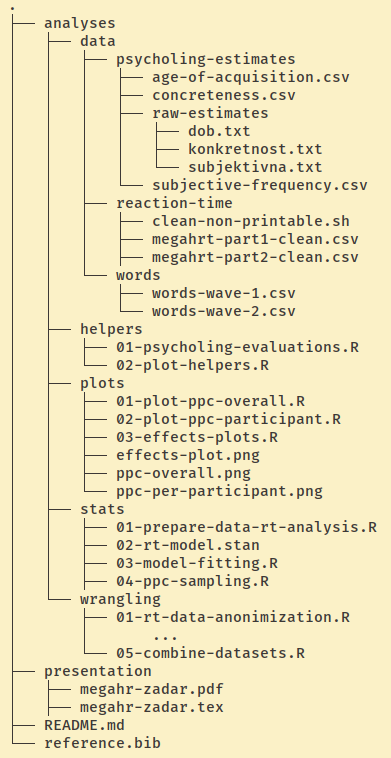
\includegraphics[scale=.25]{images/tree-light.png}
        \end{columns}
    \end{frame}
\end{noheadline}

\section{Upravljanje istraživačkim podacima}

\begin{noheadline}
    \begin{frame}
        \sectionpage

        \begin{center}
            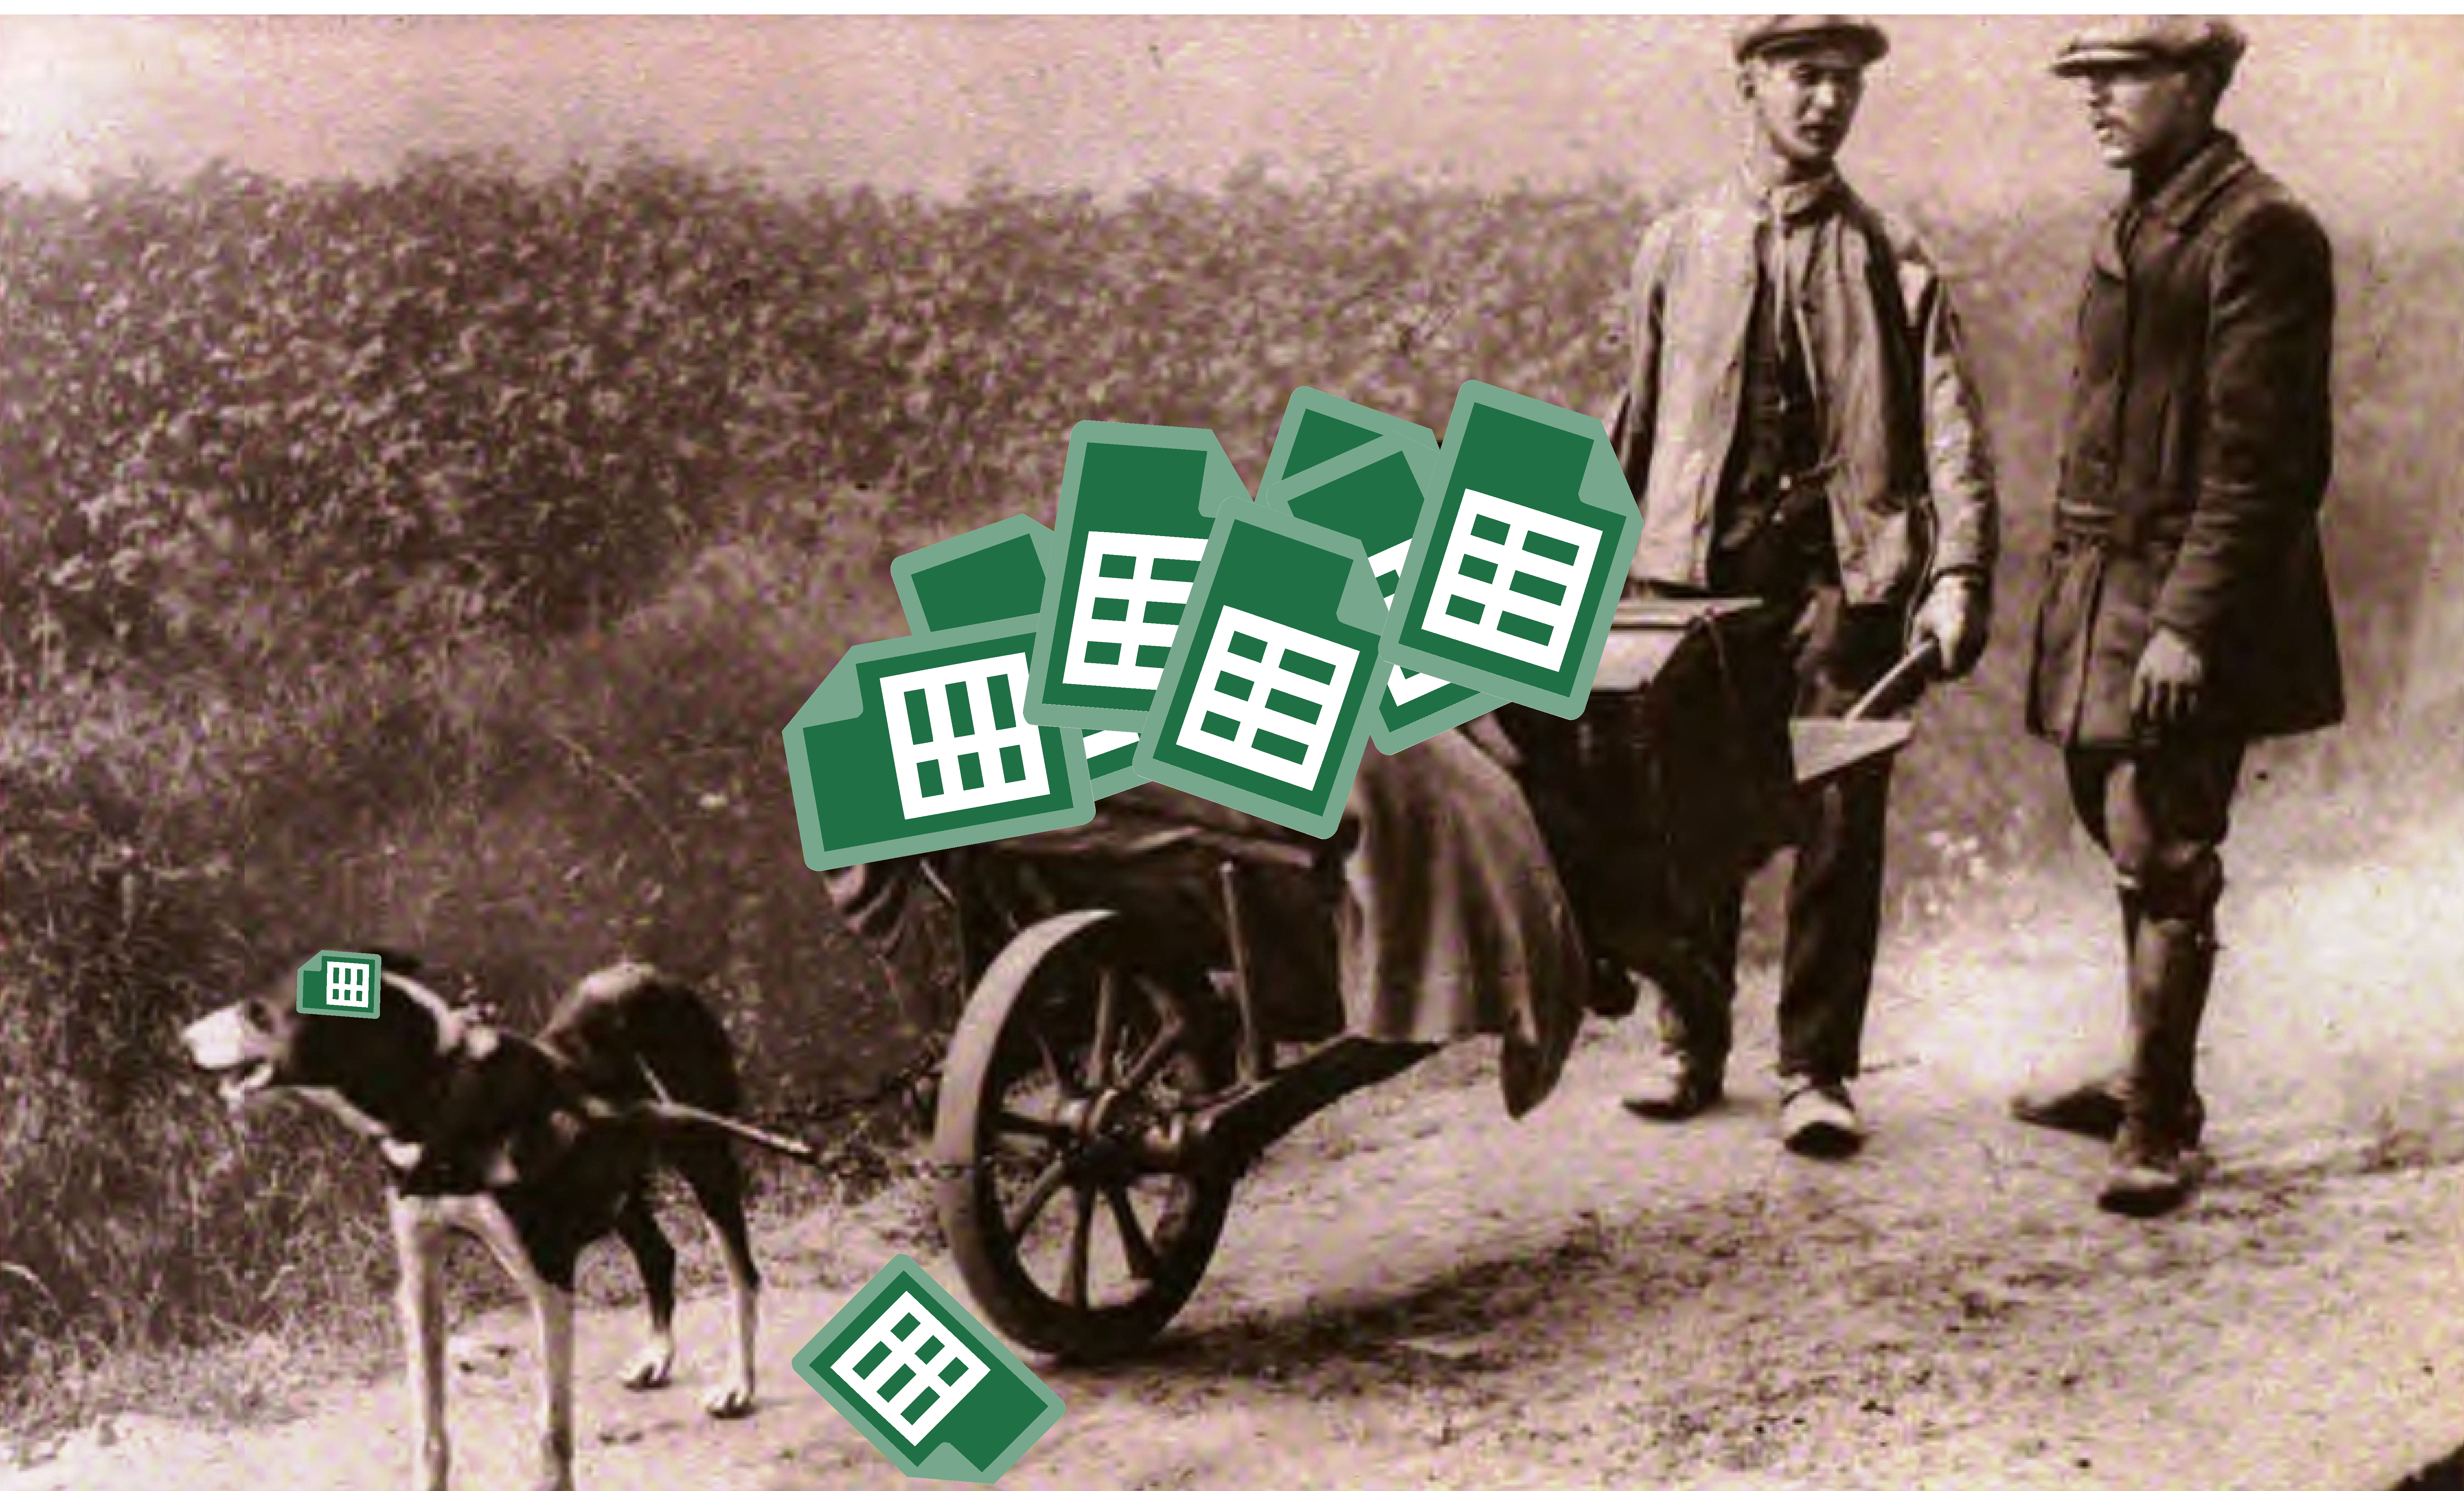
\includegraphics[scale=.05]{images/peasant-folder.pdf}
        \end{center}
    \end{frame}
\end{noheadline}

\begin{noheadline}
    \begin{frame}
        \frametitle{Upravljanje istraživačkim podacima}

        \begin{itemize}
            \setlength{\itemsep}{2em}

            \item spremite sirove podatke!

            \begin{itemize}
                \item pohranite ih na sigurno mjesto

                \item onemogućite izmjenu podataka (read-only)

                \item nemojte ih zamijeniti pročišćenim podacima
            \end{itemize}

            \pause

            \item napravite sigurnosne kopije, i pohranite ih na nekoliko
                različitih mjesta

            \pause

            \item koristite otvorene formate za pohranu

            \begin{itemize}
                \item primjerice \texttt{CSV} (comma separated values) umjesto
                    \texttt{XLSX}
            \end{itemize}
        \end{itemize}
    \end{frame}
\end{noheadline}

\begin{frame}
    \begin{itemize}
        \setlength{\itemsep}{2em}

        \item napravite uredne (\textit{tidy}) podatke

        \begin{itemize}
            \item svaki stupac je jedna varijabla (ne spajati dvije vrijednosti
                u isti stupac)

            \item svaki red je jedno opažanje/jedinica analize

            \item ne ostavljajte prazne ćelije
        \end{itemize}

        \pause

        \item bilježite sve korake procesiranja skupa podataka

        \pause

        \begin{itemize}
            \item procesiranje podataka je jedan od ključnih koraka u analizi

            \pause

            \item mora biti moguće pratiti postupak od sirovih podataka do
                podataka korištenih u obradama
        \end{itemize}

        \pause

        \item arhivirajte podatke u uglednom repozitoriju (CROSSDA, Zenodo)
    \end{itemize}
\end{frame}

\section{Praćenje promjena}

\begin{noheadline}
    \begin{frame}
        \sectionpage

        \begin{center}
            
\includegraphics[scale=.20]{images/phdcomics-filenaming.png}
        \end{center}
    \end{frame}
\end{noheadline}

\begin{noheadline}
    \begin{frame}
        \frametitle{Praćenje promjena}

        \begin{itemize}
            \setlength{\itemsep}{2em}

            \item olakšava praćenje istraživačkog procesa

            \begin{itemize}
                \item kad je nastala promjena u nekom dokumentu

                \item vraćanje na starije verzije
            \end{itemize}

            \pause

            \item olakšava reproduciranje postupaka koji su doveli do nekog
                ishoda (npr. istraživački rad, izvještaj)

            \pause

            \item specijalizirani alati (\texttt{git}) i servisi (GitHub) ili
                ručno

        \end{itemize}
    \end{frame}
\end{noheadline}

\subsection{Ručno praćenje promjena}

\begin{frame}[fragile]
    \begin{itemize}
        \setlength{\itemsep}{2em}

        \item u folder projekta dodati \texttt{CHANGELOG.txt} dokument

        \begin{itemize}
            \item bilješke s izmjenama učinjenima na datotekama projekta
            \item svaki unos ima vremensku oznaku, najnoviji unosi na početku
        \end{itemize}

        \pause

        \begin{lstlisting}
    #### [05-11-2020_12-00]
    - prosirio primjer za rucno pracenje izmjena
    - dodao slike
    #### [05-11-2020_11-15]
    - dodao primjer za rucno pracenje izmjena
        \end{lstlisting}

    \end{itemize}
\end{frame}

\begin{frame}[fragile]
    \begin{itemize}
        \setlength{\itemsep}{2em}

        \item napravite kopiju projekta kad god učinite neku značajnu promjenu

        \pause

        \item kopiju pohranite u folder unutar projektnog foldera

        \item kao ime foldera s kopijom stavite datum kad je kopija napravljena

        \pause

        \begin{lstlisting}
    projekt/
    |-- trenutna
    |-- 05-11-2020
    |-- 04-11-2020
        \end{lstlisting}

        \pause

        \item memorija je jeftina, podaci su skupi!
    \end{itemize}
\end{frame}

\subsection{Savjeti}

\begin{frame}
    \begin{itemize}
        \setlength{\itemsep}{2em}

        \item male promjene --- skupina izmjena koje biste u nekom trenu
            mogli poželjeti poništiti

        \pause

        \item često dijelite i usklađujte izmjene

        \pause

        \item pazite na to da samo jedna osoba u danom trenutku radi na nekoj
            datoteci!
    \end{itemize}
\end{frame}

\section{Dodatni materijali}

\begin{noheadline}
    \begin{frame}
        \frametitle{Dodatni materijali}
    \end{frame}
\end{noheadline}

\end{document}
